%------------------------------------------------------------------------------
% CV in Latex
% Author : Charles Rambo
% 2nd Author: Marcin Kurtz
% Based off of: https://github.com/sb2nov/resume and Jake's Resume on Overleaf
% Most recently updated version may be found at https://github.com/fizixmastr 
% License : MIT
%------------------------------------------------------------------------------

\documentclass[A4,11pt]{article}
%\documentclass[letterpaper,11pt]{article} %For use in US
\usepackage{latexsym}
\usepackage[empty]{fullpage}
\usepackage{titlesec}
\usepackage{marvosym}
\usepackage[usenames,dvipsnames]{color}
\usepackage{verbatim}
\usepackage{enumitem}
\usepackage[hidelinks]{hyperref}
\usepackage[english]{babel}
\usepackage{tabularx}
\usepackage{tikz}
\input{glyphtounicode}

%-----FONT OPTIONS-------------------------------------------------------------
% serif
 \usepackage{palatino}
% \usepackage{times} %This is the default as well
% \usepackage{charter}

% sans-serif
% \usepackage{helvet}
% \usepackage[sfdefault]{noto-sans}
% \usepackage[default]{sourcesanspro}

%-----PAGE SETUP---------------------------------------------------------------

% Adjust margins
\addtolength{\oddsidemargin}{-1cm}
\addtolength{\evensidemargin}{-1cm}
\addtolength{\textwidth}{2cm}
\addtolength{\topmargin}{-1cm}
\addtolength{\textheight}{2cm}

% Margins for US Letter size
%\addtolength{\oddsidemargin}{-0.5in}
%\addtolength{\evensidemargin}{-0.5in}
%\addtolength{\textwidth}{1in}
%\addtolength{\topmargin}{-.5in}
%\addtolength{\textheight}{1.0in}

\urlstyle{same}

\raggedbottom
\raggedright
\setlength{\tabcolsep}{0cm}

% Sections formatting
\titleformat{\section}{
  \vspace{-4pt}\scshape\raggedright\large
}{}{0em}{}[\color{black}\titlerule \vspace{-5pt}]

% Ensure that .pdf is machine readable/ATS parsable
\pdfgentounicode=1

%-----CUSTOM COMMANDS FOR FORMATTING SECTIONS----------------------------------
\newcommand{\CVItem}[1]{
  \item\small{
    {#1 \vspace{-2pt}}
  }
}

\newcommand{\CVSubheading}[4]{
  \vspace{-2pt}\item
    \begin{tabular*}{0.97\textwidth}[t]{l@{\extracolsep{\fill}}r}
      \textbf{#1} & #2 \\
      \small#3 & \small #4 \\
    \end{tabular*}\vspace{-7pt}
}

\newcommand{\CVSubSubheading}[2]{
    \item
    \begin{tabular*}{0.97\textwidth}{l@{\extracolsep{\fill}}r}
      \text{\small#1} & \text{\small #2} \\
    \end{tabular*}\vspace{-7pt}
}

\newcommand{\CVSubItem}[1]{\CVItem{#1}\vspace{-4pt}}

\renewcommand\labelitemii{$\vcenter{\hbox{\tiny$\bullet$}}$}

\newcommand{\CVSubHeadingListStart}{\begin{itemize}[leftmargin=0.5cm, label={}]}
% \newcommand{\resumeSubHeadingListStart}{\begin{itemize}[leftmargin=0.15in, label={}]} % Uncomment for US
\newcommand{\CVSubHeadingListEnd}{\end{itemize}}
\newcommand{\CVItemListStart}{\begin{itemize}}
\newcommand{\CVItemListEnd}{\end{itemize}\vspace{-5pt}}

%------------------------------------------------------------------------------
% CV STARTS HERE  %
%------------------------------------------------------------------------------
\begin{document}

%-----HEADING------------------------------------------------------------------

\begin{minipage}[c]{0.05\textwidth}
\-\
\end{minipage}
\begin{minipage}[c]{0.2\textwidth}
\begin{tikzpicture}
    \clip (0,0) circle (1.75cm);
    \node at (0, 0) {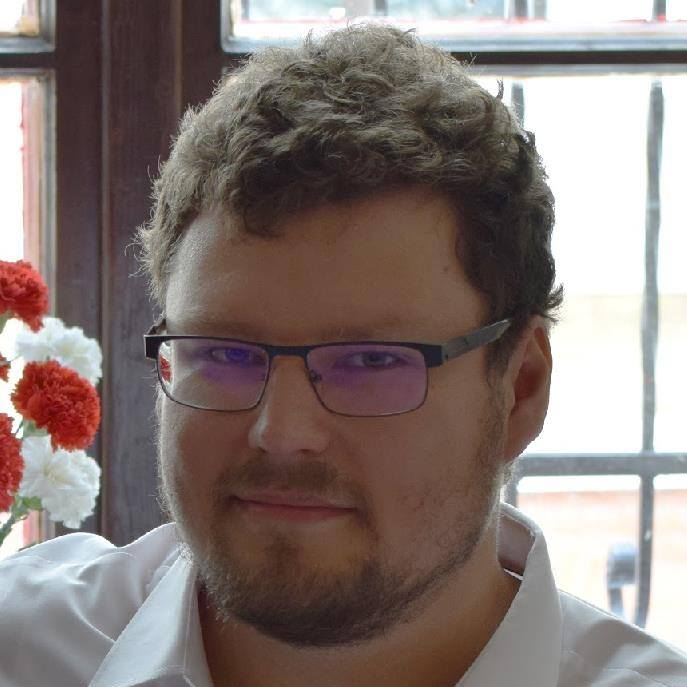
\includegraphics[width = 3.5cm]{Me}};
\end{tikzpicture}
\hfill\vline\hfill
\end{minipage}
\begin{minipage}[c]{0.4\textwidth}
    \textbf{\Huge \scshape{Marcin Kurtz}} \\ \vspace{1pt}
    \small{+48 662 466 302} \\
    \href{mailto:kurtz.marcin@gmail.com}{\underline{kurtz.marcin@gmail.com}}\\
    \href{https://www.linkedin.com/in/marcin-kurtz/}{\underline{linkedin.com/in/marcin-kurtz/}} \\
    \href{https://github.com/mkIO}{\underline{github.com/mkIO}}
\end{minipage}

\section{Bio}
Senior Fullstack Engineer and Lead Developer with over 8 years’ experience in delivering modern web applications
utilizing multiple frameworks (React, Angular) with the latest .NET framework, together with implementing DevOps solutions targeting Azure Cloud and on-premise solutions.

%-----EDUCATION----------------------------------------------------------------
\section{Education}
  \CVSubHeadingListStart
    \CVSubheading
      {{Bachelor of Engineering $|$ \emph{\small{Informatics}}}}{2011 -- 2015}
      {Faculty of Applied Mathematics, Silesian University of Technology}{Gliwice, Poland}
    \CVSubheading
      {{Master of Engineering $|$ \emph{\small{Applied Mathematics and Cryptography}}}}{2007 -- 2014}
      {Faculty of Applied Mathematics, Silesian University of Technology}{Gliwice, Poland}
  \CVSubHeadingListEnd

%-----WORK EXPERIENCE----------------------------------------------------------

\section{Work Experience}
  \CVSubHeadingListStart
    \CVSubheading
      {Lead Developer}{01/2021 - present}
      {Future Processing Sp. z o.o.}{Gliwice, Poland}
      \CVItemListStart
        \CVItem{\textbf{Responsibilites}: Designing the architecture of software products and APIs, software development, implementing devops infrastructure, bug fixing and refactoring, developing new business critical features, core review}
        \CVItem{\textbf{Technologies}: : C\#, TypeScript, Powershell, .NET Core/5/6, React, REST API Services, Azure Cloud Services/Functions, Azure SDK, Azure SQL Server, Azure Service Bus, Terraform}
      \CVItemListEnd
    \CVSubheading
      {Senior Software Developer}{07/2018 - 01/2021}
      {Future Processing Sp. z o.o.}{Gliwice, Poland}
      \CVItemListStart
        \CVItem{\textbf{Responsibilites}: Designing the architecture of software products and APIs, software development, bug fixing and refactoring, developing new business critical features, code review}
        \CVItem{\textbf{Technologies}: .NET Core, Angular, Powershell, REST API Services, Azure Services, Azure DevOps and Octopus Deployment pipelines, C\#, TypeScript, Azure SQL Server, Azure Service Bus, OData Services}
      \CVItemListEnd
    \CVSubheading
      {Medium Software Developer}{07/2014 - 07/2018}
      {Future Processing Sp. z o.o.}{Gliwice, Poland}
      \CVItemListStart
        \CVItem{\textbf{Responsibilites}: 
        Application development, bug fixing, developing new business critical features, refactoring, code review, implementing backend services}
        \CVItem{\textbf{Technologies}: ASP.NET, NET 4.7, WCF, XSLT with XML, SQL Server, VB.NET, C\#, Chef}
      \CVItemListEnd
    \CVSubheading
      {Junior Software Developer}{07/2013 - 06/2014}
      {Future Processing Sp. z o.o.}{Gliwice, Poland}
      \CVItemListStart
        \CVItem{Application development}
        \CVItem{\textbf{Technologies}: ASP.NET, NET 4, WCF, SQL Server, XML with XML, VB.NET, C\#, JavaScript}
      \CVItemListEnd
  \CVSubHeadingListEnd

%----- CERTIFICATES --------------------------------------------------------
\section{Certificates}
  \CVSubHeadingListStart
    \CVSubheading
      {AZ-204: Developing Solutions for Microsoft Azure}{01/2022}
      {Developing Solutions for Microsoft Azure}{}
    \CVSubheading
      {70-486: Developing ASP .NET 4.5 MVC Web Applications}{12/2015}
      {Developing ASP .NET 4.5 MVC Web Applications}{}
    \CVSubheading
      {70-480: Programming in HTML 5 with JavaScript and CSS3}{07/2015}
      {HTML 5 with JavaScript and CSS3}{}
    \CVSubheading
      {M101N: MongoDB for .NET Developers}{06/2015}
      {Developing MongoDB solutions for .NET applications}{}
  \CVSubHeadingListEnd

%-----SKILLS-------------------------------------------------------------------
\section{Skills}
  \CVSubHeadingListStart
    \CVSubheading
      {Languages}{}
      {Polish (native), English (B1), French (A1)}{}
    \CVSubheading
      {Document Creation}{}
      {Microsoft Office Suite, LaTex, Markdown}{}
    \CVSubheading
      {Web technologies}{}
      {ASP.NET, .NET, HTML5, CSS, SASS, Less, JavaScript, Typescript, React, Angular, Kendo UI, \\
      REST API, ASP Core Web API, .NET Minimal API, ASP Core MVC, Razor, Razor Pages,\\
      Singnal R, OAuth, Open Connect, Azure AD, Azure B2C, Auth0, One Login, RxJS,\\
      Entity Framework, NoSQL databases}{}
    \CVSubheading
      {Cloud}{}
      {Azure Services, Azure CLI, Azure RM, Cognitive Services, Service Bus, Serverless,\\
      Azure SQL, Cosmos DB, Azure Front Door, VNET and security, Chef, Terraform.}{}
    \CVSubheading
      {Mobile}{}
      {Xamarin, .NET Maui}{}
    \CVSubheading
      {Languages}{}
      {C\#, TypeScript, Javascript, Powershell.}{}
    \CVSubheading
      {Tools}{}
      {Visual Studio, ReSharper, VS Code, Rider, Docker, Git, Azure DevOps, GitHub, RabbitMQ.}{}
    \CVSubheading
      {Architecture}{}
      {Designing solution architecture, on premise/cloud based.\\
      Supporting client with architecture decisions, mentoring with proper implementation.}{},
    \CVSubheading
      {Practices}{}
      {Domain Driven Design, CQS, CQRS, TDD, Aspect Oriented programing, reactive programing, functional programing.}{}
  \CVSubHeadingListEnd  
    
%------------------------------------------------------------------------------
\end{document}